% !TEX root =  ./main.tex

\section{Semantic correspondence}

In this paper, we claim, but do not prove, that the \GROOVE semantics correctly captures the Reaction Systems transitions recalled in \Cref{sec:RS}. A complete formal proof is outside the scope of this paper, which focusses on experimental results; however, in this section we provide a sketch of such a proof.

As described in \Cref{sec:RS2GTS}, each GROOVE state is a graph consisting of a fixed part (which is the same in every state) and a variable part. The fixed part contains an encoding of
\begin{enumerate*}[label=\emph{(\roman*)}]
\item the reaction system $\cal A$ itself, with the entities $S$ given as \Entity-typed nodes, and
\item the automata of the context processes, with individual processes corresponding to \Token-typed nodes and states given as \State-typed nodes.
\end{enumerate*} 
The variable part consisting of \present flags on \Entity nodes and a \current-edge from every \Token to a \State. An RS state $[\mathsf{M}]$, on the other hand, consists of
%
\begin{enumerate*}[label=\emph{(\roman*)}]
\item sets $D$ of currently present entities,
\item fixed reactions $(R,I,P)$, and
\item regular context processes $\mathsf K$.
\end{enumerate*}

A \GROOVE state $G$ is equivalent to an RS state $[\mathsf{M}]$ if:
%
\begin{enumerate*}[label=\emph{(\roman*)}]
\item the union of all $D$ in $[\mathsf{M}]$ corresponds precisely to the set of \Entity nodes that are flagged as \present in a $G$, and
\item there is a one-to-one correspondence of the $\mathsf K$ in $[\mathsf{M}]$ and the $\Token$-nodes in $G$, such that the \current state of that \Token is the start state of the automaton for $\mathsf K$.
\end{enumerate*}

We claim that this equivalence establishes a bisimulation between the \GROOVE and RS state spaces. (It is not an isomorphism for two reasons:
%
\begin{enumerate*}[label=\emph{(\roman*)}]
\item $\mathsf{[M]}$ may contain multiple, overlapping sets $D$ whereas $G$ merely encodes their union;
\item the RS semantics for $\textsf K$ ``consumes'' the process (rules \textit{(Cxt)}--\textit{(Rec)} in \Cref{fig:guardforRS2nd}) whereas $G$ keeps the automaton intact, merely moving the \current pointer.
\end{enumerate*}
%
To prove this claim, we have to show correspondence of the transitions.

Concretely, every $\obs{\obs{D}{R',I',C}}{R,I,P}$-labelled transition corresponds to single application of the recipe \fireR, which in turn consists of applications of rules \contextR (see \Cref{fig:context}) followed by \reactR (see \Cref{fig:react}).
%
\begin{figure}
\centering
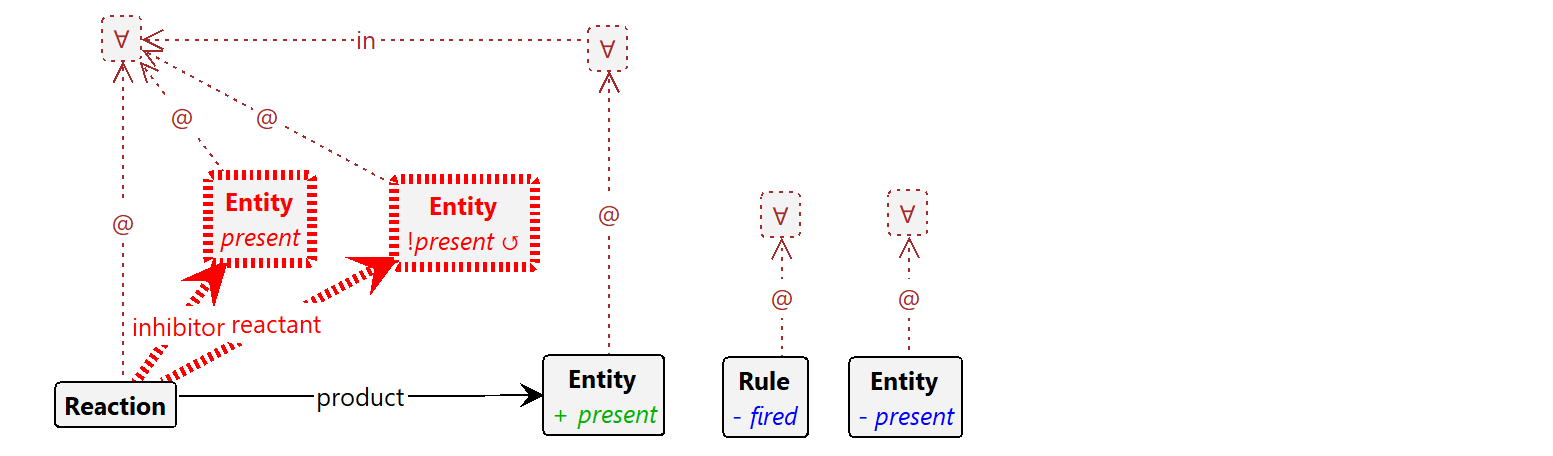
\includegraphics[scale=.2]{figs/react}
\caption{Rule for reaction firing}
\label{fig:react}
\end{figure}
%
Both of these rules are universally quantified. Roughly speaking, referring to \Cref{fig:guardforRS2nd}, \contextR simultaneously encodes all sub-transitions of the form
%
\[\begin{array}{rcll}
D & \xrightarrow{\obs{\obs{D}{\emptyset,\emptyset,\emptyset}}
                     {\emptyset,\emptyset,\emptyset}} & D'
  & \quad\text{\small{(rule (\textit{Ent}))}} \\
\mathsf K
  & \xrightarrow{\obs{\obs{\emptyset}{R',I',C}}
                     {\emptyset,\emptyset,\emptyset}} & \mathsf K'
  & \quad\text{\small{(rules (\textit{Cxt})--(\textit{Rec}))}}
\end{array}\]
%
as well as their composition and filtering (rules (\textit{Par})--(\textit{Sys})). \reactR in turns simultaneously encodes all sub-transitions of the form
%
\[\begin{array}{rcll}
(R,I,P)
  & \xrightarrow{\obs{\obs{\emptyset}
                     {\emptyset,\emptyset,\emptyset}}{R',I',P'}} & \mathsf M'
  & \enspace\text{\small{(rules (\textit{Pro})--(\textit{Inh}))}}
\end{array}\]
%
together with their composition with the \contextR-transitions (rule (\textit{Par})) and filtering (rule (\textit{Sys})). (The \fired-flags on the \Step-nodes, added by \contextR and removed again by \reactR, play no role in this correspondence: for the purpose of the equivalence of the \GROOVE and RS semantics, they might be omitted entirely.)

\section{Auxiliary Material}

\subsection{Auxiliary Material for the toy running example}\label{app:running}

The \BioResolve specification for the toy running example about the interaction between the student and the vending machine is reported in \Cref{fig:bioresolve:toy}. The corresponding RS has been described in \Cref{sec:student} and it has been used to illustrate some key features of the \GROOVE encoding in \Cref{sec:RS2GTS}.

\begin{figure}[t]
\begin{minipage}{0.9\linewidth}
\footnotesize
\begin{verbatim}
myentities([cpowder,tpowder]). % initial set D0

myreactions([                  % list of reactions
    react([idle],[am],[am]),
    react([am],[idle],[am]),
    react([ccoin,cpowder],[nomilk],[cappuccino]),
    react([ccoin,cpowder,nomilk],[],[espresso]),
    react([tcoin,tpowder],[],[tea]),
    react([cpowder],[],[cpowder]),
    react([tpowder],[],[tpowder]),
    react([anger],[],[bang]) ]).

mycontext("[refill,student]"). % context processes

myenvironment("[               % context definitions
    refill = ({nomilk}.refill 
            + {}.refill),
    student = (?{},{am},{tcoin}?.gettea 
             + ?{am},{},{ccoin}?.getcappuccino 
             + {idle}.student),
    gettea = (?{tea},{},{}?.student
            + ?{},{tea},{anger}?.student),
    getcappuccino = (?{cappuccino},{},{}?.student 
                    + ?{espresso},{},{anger}?.student) ]").
\end{verbatim}
\end{minipage}
\caption{\BioResolve implementation of the vending machine RS from \Cref{sec:student}. The question marks \texttt{?} are used to delimit guarded prefixes in context processes.}
\label{fig:bioresolve:toy}
\end{figure}

\subsection{Auxiliary Material for the Comorbidity Case Study}

\newcommand{\ent}[1]{\mathsf{#1}}
\newcommand{\ents}[2]{\mathsf{#1}\texttt{\_}\mathsf{#2}}

The RS specification for the comorbidity case study presented in~\cite{DBLP:conf/cmsb/BowlesBBFGM24} is reported in \Cref{fig:bioresolve:comorbidities:reactions} (set of reactions) and \Cref{fig:bioresolve:comorbidities:contexts} (context processes definitions), where we assume the initial state is $\mathsf{D}_0  =  \varnothing$.
The corresponding experimentation with \GROOVE has been discussed in \Cref{sec:cmsb2024}.

\begin{figure*}[t]
\fontsize{6}{0}
\[
\begin{array}{rcl}
\mathsf{Feats} &  \triangleq 
& (\{\ent{hyper}\},\varnothing,\{\ent{hyper}\})
\mid  (\{\mathsf{afib}\},\varnothing,\{\ent{afib}\})
\mid  (\{\ents{has}{fib}\},\varnothing,\{\ents{has}{fib}\})
\mid  (\{\ents{heart}{rate}\},\varnothing,\{\ents{heart}{rate}\})
\mid  (\{\ents{consensus}{acei}\},\varnothing,\{\ents{consensus}{acei}\})
\\[-4pt] & \mid &  (\{\ent{over75}\},\varnothing,\{\ent{over75}\})
\mid  (\{\ent{below55}\},\varnothing,\{\ent{below55}\})
\mid  (\{\ent{diabete}\},\varnothing,\{\ent{diabete}\})
\mid  (\{\ent{origin}\},\varnothing,\{\ent{origin}\})
\\[-4pt] & \mid &  (\{\ents{doac}{int}\},\varnothing,\{\ents{doac}{int}\})
\mid  (\{\ent{hyper}\},\varnothing,\{\ent{diseases}\})
\mid  (\{\ent{diabete}\},\varnothing,\{\ent{diseases}\})
\\[-4pt]
\mathsf{Drugs} &  \triangleq 
& (\{\ents{get}{diltiazem}\},\{\ents{stop}{cbb}\},\{\ent{diltiazem},\ent{cbb}\})
\mid  (\{\ent{diltiazem}\},\{\ents{stop}{cbb}\},\{\ent{diltiazem},\ent{cbb}\})
\mid  (\{\ents{get}{verapamil}\},\{\ents{stop}{cbb}\},\{\ent{verapamil},\ent{cbb}\})
\\[-4pt] & \mid &  (\{\ent{verapamil}\},\{\ents{stop}{cbb}\},\{\ent{verapamil},\ent{cbb}\})
\mid  (\{\ent{diltiazem},\ent{verapamil}\},\{\ents{stop}{cbb}\},\{\ents{alert}{dup}\})
%
\mid  (\{\ents{get}{propranolol}\},\{\ents{stop}{nsbb}\},\{\ent{propranolol},\ent{nsbb}\})
\\[-4pt] & \mid &  (\{\ent{propranolol}\},\{\ents{stop}{nsbb}\},\{\ent{propranolol},\ent{nsbb}\})
\mid  (\{\ents{get}{carvedilol}\},\{\ents{stop}{nsbb}\},\{\ent{carvedilol},\ent{nsbb}\})
\mid  (\{\ent{carvedilol}\},\{\ents{stop}{nsbb}\},\{\ent{carvedilol},\ent{nsbb}\})
\\[-4pt] & \mid &  (\{\ent{propranolol},\ent{carvedilol}\},\{\ents{stop}{nsbb}\},\{\ents{alert}{dup}\})
%
\mid  (\{\ents{get}{bisoprolol}\},\{\ents{stop}{sbb}\},\{\ent{bisoprolol},\ent{sbb}\})
\mid  (\{\ent{bisoprolol}\},\{\ents{stop}{sbb}\},\{\ent{bisoprolol},\ent{sbb}\})
\\[-4pt] & \mid &  (\{\ents{get}{atenolol}\},\{\ents{stop}{sbb}\},\{\ent{atenolol},\ent{sbb}\})
\mid  (\{\ent{atenolol}\},\{\ents{stop}{sbb}\},\{\ent{atenolol},\ent{sbb}\})
\mid  (\{\ent{bisoprolol},\ent{atenolol}\},\{\ents{stop}{sbb}\},\{\ents{alert}{dup}\})
%
\\[-4pt] & \mid &  (\{\ents{get}{flecainide}\},\{\ents{stop}{flec}\},\{\ent{flecainide}\})
\mid  (\{\ent{flecainide}\},\{\ents{stop}{flec}\},\{\ent{flecainide}\})
\mid  (\{\ents{get}{warfarin}\},\{\ents{stop}{warf}\},\{\ent{warfarin}\})
\\[-4pt] & \mid &  (\{\ent{warfarin}\},\{\ents{stop}{warf}\},\{\ent{warfarin}\})
%
\mid  (\{\ents{get}{apixaban}\},\{\ents{stop}{doac}\},\{\ent{apixaban},\ent{doac}\})
\mid  (\{\ent{apixaban}\},\{\ents{stop}{doac}\},\{\ent{apixaban},\ent{doac}\})
\\[-4pt] & \mid &  (\{\ents{get}{dabigatran}\},\{\ents{stop}{doac}\},\{\ent{dabigatran},\ent{doac}\})
\mid  (\{\ent{dabigatran}\},\{\ents{stop}{doac}\},\{\ent{dabigatran},\ent{doac}\})
\mid  (\{\ent{apixaban},\ent{dabigatran}\},\{\ents{stop}{doac}\},\{\ents{alert}{dup}\})
%
\\[-4pt] & \mid &  (\{\ents{get}{vkant}\},\{\ents{stop}{vkant}\},\{\ent{vkant}\})
\mid  (\{\ent{vkant}\},\{\ents{stop}{vkant}\},\{\ent{vkant}\})
%
\mid  (\{\ents{get}{benazepril}\},\{\ents{stop}{acei}\},\{\ent{benazepril},\ent{acei}\})
\\[-4pt] & \mid &  (\{\ent{benazepril}\},\{\ents{stop}{acei}\},\{\ent{benazepril},\ent{acei}\})
\mid  (\{\ents{get}{captopril}\},\{\ents{stop}{acei}\},\{\ent{captopril},\ent{acei}\})
\mid  (\{\ent{captopril}\},\{\ents{stop}{acei}\},\{\ent{captopril},\ent{acei}\})
\\[-4pt] & \mid &  (\{\ent{benazepril},\ent{captopril}\},\{\ents{stop}{acei}\},\{\ents{alert}{dup}\})
%
\mid  (\{\ents{get}{olmesortan}\},\{\ents{stop}{arb}\},\{\ent{olmesortan},\ent{arb}\})
\mid  (\{\ent{olmesortan}\},\{\ents{stop}{arb}\},\{\ent{olmesortan},\ent{arb}\})
\\[-4pt] & \mid &  (\{\ents{get}{irbesartan}\},\{\ents{stop}{arb}\},\{\ent{irbesartan},\ent{arb}\})
\mid  (\{\ent{irbesartan}\},\{\ents{stop}{arb}\},\{\ent{irbesartan},\ent{arb}\})
\mid  (\{\ent{olmesortan},\ent{irbesartan}\},\{\ents{stop}{arb}\},\{\ents{alert}{dup}\})
%
\\[-4pt] & \mid &  (\{\ents{get}{indapamide}\},\{\ents{stop}{td}\},\{\ent{indapamide},\ent{td}\})
\mid  (\{\ent{indapamide}\},\{\ents{stop}{td}\},\{\ent{indapamide},\ent{td}\})
\mid  (\{\ents{get}{chlorothiazide}\},\{\ents{stop}{td}\},\{\ent{chlorothiazide},\ent{td}\})
\\[-4pt] & \mid &  (\{\ent{chlorothiazide}\},\{\ents{stop}{td}\},\{\ent{chlorothiazide},\ent{td}\})
\mid  (\{\ent{indapamide},\ent{chlorothiazide}\},\{\ents{stop}{td}\},\{\ents{alert}{dup}\})
%
\mid  (\{\ent{doac}\},\{\ents{doac}{ok},\ents{doac}{fail}\},\{\ents{doac}{test}\})
\\[-4pt] & \mid &  (\{\ents{doac}{ok}\},\{\ents{doac}{fail}\},\{\ents{doac}{ok}\})
\mid  (\{\ents{doac}{fail}\},\{\ents{doac}{ok}\},\{\ents{doac}{fail}\})
\mid  (\{\ent{doac}\},\{\ents{doac}{fail},\ents{stop}{doac}\},\{\ents{doac}{danger}\})
\\[-4pt] & \mid &  (\{\ent{doac}\},\{\ents{doac}{danger},\ents{stop}{doac}\},\{\ent{danger}\})
\\[-4pt]
\ent{ADR} &  \triangleq 
& (\{\ents{get}{apixaban},\ents{get}{diltiazem}\},\varnothing,\{\ent{moderate}\})
\mid  (\{\ents{get}{apixaban},\ent{diltiazem}\},\varnothing,\{\ent{moderate}\})
\mid  (\{\ent{apixaban},\ents{get}{diltiazem}\},\varnothing,\{\ent{moderate}\})
\\[-4pt] & \mid &  (\{\ent{apixaban},\ent{diltiazem}\},\varnothing,\{\ent{moderate}\})
\mid  (\{\ents{get}{apixaban},\ents{get}{verapamil}\},\varnothing,\{\ent{moderate}\})
\mid  (\{\ents{get}{apixaban},\ent{verapamil}\},\varnothing,\{\ent{moderate}\})
\\[-4pt] & \mid &  (\{\ent{apixaban},\ents{get}{verapamil}\},\varnothing,\{\ent{moderate}\})
\mid  (\{\ent{apixaban},\ent{verapamil}\},\varnothing,\{\ent{moderate}\})
\mid  (\{\ents{get}{dabigatran},\ents{get}{diltiazem}\},\varnothing,\{\ent{moderate}\})
\\[-4pt] & \mid &  (\{\ents{get}{dabigatran},\ent{diltiazem}\},\varnothing,\{\ent{moderate}\})
\mid  (\{\ent{dabigatran},\ents{get}{diltiazem}\},\varnothing,\{\ent{moderate}\})
\mid  (\{\ent{dabigatran},\ent{diltiazem}\},\varnothing,\{\ent{moderate}\})
\\[-4pt] & \mid &  (\{\ents{get}{dabigatran},\ents{get}{verapamil}\},\varnothing,\{\ent{major}\})
\mid  (\{\ents{get}{dabigatran},\ent{verapamil}\},\varnothing,\{\ent{major}\})
\mid  (\{\ent{dabigatran},\ents{get}{verapamil}\},\varnothing,\{\ent{major}\})
\\[-4pt] & \mid &  (\{\ent{dabigatran},\ent{verapamil}\},\varnothing,\{\ent{major}\})
\mid  (\{\ents{get}{dabigatran},\ents{get}{carvedilol}\},\varnothing,\{\ent{moderate}\})
\mid  (\{\ents{get}{dabigatran},\ent{carvedilol}\},\varnothing,\{\ent{moderate}\})
\\[-4pt] & \mid &  (\{\ent{dabigatran},\ents{get}{carvedilol}\},\varnothing,\{\ent{moderate}\})
\mid  (\{\ent{dabigatran},\ent{carvedilol}\},\varnothing,\{\ent{moderate}\})
\mid  (\{\ents{get}{warfarin},\ents{get}{benazepril}\},\varnothing,\{\ent{minor}\})
\\[-4pt] & \mid &  (\{\ents{get}{warfarin},\ent{benazepril}\},\varnothing,\{\ent{minor}\})
\mid  (\{\ent{warfarin},\ents{get}{benazepril}\},\varnothing,\{\ent{minor}\})
\mid  (\{\ent{warfarin},\ent{benazepril}\},\varnothing,\{\ent{minor}\})
\\[-4pt] & \mid &  (\{\ents{get}{warfarin},\ents{get}{indapamide}\},\varnothing,\{\ent{minor}\})
\mid  (\{\ents{get}{warfarin},\ent{indapamide}\},\varnothing,\{\ent{minor}\})
\mid  (\{\ent{warfarin},\ents{get}{indapamide}\},\varnothing,\{\ent{minor}\})
\\[-4pt] & \mid &  (\{\ent{warfarin},\ent{indapamide}\},\varnothing,\{\ent{minor}\})
\mid  (\{\ents{get}{warfarin},\ents{get}{chlorothiazide}\},\varnothing,\{\ent{minor}\})
\mid  (\{\ents{get}{warfarin},\ent{chlorothiazide}\},\varnothing,\{\ent{minor}\})
\\[-4pt] & \mid &  (\{\ent{warfarin},\ents{get}{chlorothiazide}\},\varnothing,\{\ent{minor}\})
\mid  (\{\ent{warfarin},\ent{chlorothiazide}\},\varnothing,\{\ent{minor}\})
\mid  (\{\ents{get}{warfarin},\ents{get}{propranolol}\},\varnothing,\{\ent{minor}\})
\\[-4pt] & \mid &  (\{\ents{get}{warfarin},\ent{propranolol}\},\varnothing,\{\ent{minor}\})
\mid  (\{\ent{warfarin},\ents{get}{propranolol}\},\varnothing,\{\ent{minor}\})
\mid  (\{\ent{warfarin},\ent{propranolol}\},\varnothing,\{\ent{minor}\})
\\[-4pt] & \mid &  (\{\ents{get}{flecainide},\ents{get}{diltiazem}\},\varnothing,\{\ent{major}\})
\mid  (\{\ents{get}{flecainide},\ent{diltiazem}\},\varnothing,\{\ent{major}\})
\mid  (\{\ent{flecainide},\ents{get}{diltiazem}\},\varnothing,\{\ent{major}\})
\\[-4pt] & \mid &  (\{\ent{flecainide},\ent{diltiazem}\},\varnothing,\{\ent{major}\})
\mid  (\{\ents{get}{flecainide},\ents{get}{verapamil}\},\varnothing,\{\ent{major}\})
\mid  (\{\ents{get}{flecainide},\ent{verapamil}\},\varnothing,\{\ent{major}\})
\\[-4pt] & \mid &  (\{\ent{flecainide},\ents{get}{verapamil}\},\varnothing,\{\ent{major}\})
\mid  (\{\ent{flecainide},\ent{verapamil}\},\varnothing,\{\ent{major}\})
\mid  (\{\ents{get}{flecainide},\ents{get}{bisoprolol}\},\varnothing,\{\ent{moderate}\})
\\[-4pt] & \mid &  (\{\ents{get}{flecainide},\ent{bisoprolol}\},\varnothing,\{\ent{moderate}\})
\mid  (\{\ent{flecainide},\ents{get}{bisoprolol}\},\varnothing,\{\ent{moderate}\})
\mid  (\{\ent{flecainide},\ent{bisoprolol}\},\varnothing,\{\ent{moderate}\})
\\[-4pt] & \mid &  (\{\ents{get}{flecainide},\ents{get}{atenolol}\},\varnothing,\{\ent{moderate}\})
\mid  (\{\ents{get}{flecainide},\ent{atenolol}\},\varnothing,\{\ent{moderate}\})
\mid  (\{\ent{flecainide},\ents{get}{atenolol}\},\varnothing,\{\ent{moderate}\})
\\[-4pt] & \mid &  (\{\ent{flecainide},\ent{atenolol}\},\varnothing,\{\ent{moderate}\})
\mid  (\{\ents{get}{flecainide},\ents{get}{propranolol}\},\varnothing,\{\ent{moderate}\})
\mid  (\{\ents{get}{flecainide},\ent{propranolol}\},\varnothing,\{\ent{moderate}\})
\\[-4pt] & \mid &  (\{\ent{flecainide},\ents{get}{propranolol}\},\varnothing,\{\ent{moderate}\})
\mid  (\{\ent{flecainide},\ent{propranolol}\},\varnothing,\{\ent{moderate}\})
\mid  (\{\ents{get}{flecainide},\ents{get}{carvedilol}\},\varnothing,\{\ent{moderate}\})
\\[-4pt] & \mid &  (\{\ents{get}{flecainide},\ent{carvedilol}\},\varnothing,\{\ent{moderate}\})
\mid  (\{\ent{flecainide},\ents{get}{carvedilol}\},\varnothing,\{\ent{moderate}\})
\mid  (\{\ent{flecainide},\ent{carvedilol}\},\varnothing,\{\ent{moderate}\})
\\[-4pt] & \mid &  (\{\ent{major}\},\varnothing,\{\ent{major}\})
\mid  (\{\ent{moderate}\},\varnothing,\{\ent{moderate}\})
\mid  (\{\ent{minor}\},\varnothing,\{\ent{minor}\})
\mid  (\{\ents{alert}{dup}\},\varnothing,\{\ents{alert}{dup}\})
\mid  (\{\ent{danger}\},\varnothing,\{\ent{danger}\})
\end{array}
\]
\normalsize
\caption{Reactions for the comorbidity case study in~\Cref{sec:cmsb2024}.}
\label{fig:bioresolve:comorbidities:reactions}
\end{figure*}

\begin{figure*}[t]
\fontsize{6}{0}
\[
\begin{array}{rcl}
\ent{eafib1} &  \triangleq 
& (\varnothing,\{\ent{afib}\},\varnothing).\ent{eafib1} 
+ (\{\ent{afib}\},\varnothing,\varnothing).\ent{ehr}
\\[-4pt]
\ent{ehr} &  \triangleq 
& (\varnothing,\{\ents{heart}{rate}\},\varnothing).\ent{ehr} 
+ (\{\ents{heart}{rate}\},\varnothing,\varnothing).\ent{ebb}
\\[-4pt]
\ent{ebb} &  \triangleq 
& \varnothing.\ent{ebb} + \ents{e}{cbb} + \ents{e}{nsbb} + \ents{e}{sbb}
\\[-4pt]
\ents{e}{cbb} &  \triangleq 
& (\varnothing,\{\ent{verapamil}\},\{\ents{get}{diltiazem}\}).\ent{empty} 
+ (\varnothing,\{\ent{diltiazem}\},\{\ents{get}{verapamil}\}).\ent{empty}
\\[-4pt]
\ents{e}{nsbb} &  \triangleq 
& (\varnothing,\{\ent{carvedilol}\},\{\ents{get}{propranolol}\}).\ent{empty} 
+ (\varnothing,\{\ent{propranolol}\},\{\ents{get}{carvedilol}\}).\ent{empty}
\\[-4pt]
\ents{e}{sbb} &  \triangleq 
& (\varnothing,\{\ent{atenolol}\},\{\ents{get}{bisoprolol}\}).\ent{empty} 
+ (\varnothing,\{\ent{bisoprolol}\},\{\ents{get}{atenolol}\}).\ent{empty}
\\[-4pt]
\ent{eafib2} &  \triangleq 
& (\varnothing,\{\ent{afib}\},\varnothing).\ent{eafib2} 
+ (\{\ent{afib}\},\varnothing,\varnothing).\ent{ehf}
\\[-4pt]
\ent{ehf} &  \triangleq 
& (\varnothing,\{\ents{has}{fib}\},\varnothing).\ent{ehf} 
+ (\{\ents{has}{fib}\},\varnothing,\varnothing).\ent{eflec}
\\[-4pt]
\ent{eflec} &  \triangleq 
& \varnothing.\ent{eflec} + \ents{e}{flec}
\\[-4pt]
\ents{e}{flec} &  \triangleq 
& \{\ents{get}{flecainide}\}.\ent{empty}
\\[-4pt]
\ent{eafib3} &  \triangleq 
& (\varnothing,\{\ent{afib}\},\varnothing).\ent{eafib3} 
+ (\{\ent{afib}\},\varnothing,\varnothing).\ent{econs}
\\[-4pt]
\ent{econs} &  \triangleq 
& (\varnothing,\{\ents{heart}\ent{rate},\ents{has}{fib}\},\varnothing).\ent{econs} 
+ (\varnothing,\{\ents{consensus}{acei}\},\varnothing).\ent{econs} 
+ (\{\ents{consensus}{acei},\ents{heart}{rate}\},\varnothing,\varnothing).\ent{estroke} 
+ (\{\ents{consensus}{acei},\ents{has}{fib}\},\varnothing,\varnothing).\ent{estroke} 
\\[-4pt]
\ent{estroke} &  \triangleq 
& (\varnothing,\{\ent{diseases},\ent{over75}\},\varnothing).\ent{ewarf} 
+ (\{\ent{over75}\},\{\ents{doac}{fail},\ents{doac}{int}\},\varnothing).\ent{edoac} 
+ (\{\ent{diseases}\},\{\ents{doac}{fail},\ents{doac}{int}\},\varnothing).\ent{edoac} 
+ (\{\ent{over75},\ents{doac}{fail}\},\varnothing,\varnothing).\ent{evkant} 
\\[-4pt] 
& + & (\{\ent{over75},\ents{doac}{int}\},\varnothing,\varnothing).\ent{evkant} 
+ (\{\ent{diseases}\},\{\ents{doac}{fail},\varnothing,\varnothing).\ent{evkant} 
+ (\{\ent{diseases}\},\{\ents{doac}{int},\varnothing,\varnothing).\ent{evkant}
\\[-4pt]
\ent{ewarf} &  \triangleq 
& \varnothing.\ent{ewarf} + \ents{e}{warf}
\\[-4pt]
\ents{e}{warf} &  \triangleq 
& \{\ents{get}{warfarin}\}.\ent{empty}
\\[-4pt]
\ent{edoac} &  \triangleq 
& \varnothing.\ent{edoac} + \ents{e}{doac}
\\[-4pt]
\ents{e}{doac} &  \triangleq 
& (\varnothing,\{\ent{dabigatran}\},\{\ents{get}{apixaban}\}).\ents{e}{doacfail} 
+ (\varnothing,\{\ent{apixaban}\},\{\ents{get}{dabigatran}\}).\ents{e}{doacfail}
\\[-4pt]
\ents{e}{doacfail} &  \triangleq 
& (\{\ents{doac}{fail}\},\varnothing,\{\ents{stop}{doac}\}).\ent{evkant} 
+ (\varnothing,\{\ents{doac}{fail}\},\varnothing).\ents{e}{doacfail}
\\[-4pt]
\ent{evkant} &  \triangleq 
& \varnothing.\ent{evkant} + \ents{e}{vkant}
\\[-4pt]
\ents{e}{vkant} &  \triangleq 
& \{\ents{get}{vkant}\}.\ent{empty}
\\[-4pt]
\ent{ghyper} &  \triangleq 
& (\varnothing,\{\ent{hyper}\},\varnothing).\ent{ghyper} 
+ (\{\ent{hyper}\},\varnothing,\varnothing).\ent{g1}
\\[-4pt]
\ent{g1} &  \triangleq 
& (\{\ent{diabete}\},\varnothing,\varnothing).\ent{g2} 
+ (\{\ent{below55}\},\{\ent{diabete},\ent{origin}\},\varnothing).\ent{g2} 
+ (\varnothing,\{\ent{below55},\ent{diabete}\},\varnothing).\ent{g3} 
+ (\{\ent{origin}\},\{\ent{diabete}\},\varnothing).\ent{g3}
\\[-4pt]
\ent{g2} &  \triangleq 
& \varnothing.\ent{g2} 
+ (\varnothing,\{\ent{captopril}\},\{\ents{get}{benazepril}\}).\ent{g4}
+ (\varnothing,\{\ent{benazepril}\},\{\ents{get}{captopril}\}).\ent{g4}
+ (\varnothing,\{\ent{irbesartan}\},\{\ents{get}{olmesortan}\}).\ent{g5}
\\[-4pt]
& + & (\varnothing,\{\ent{olmesortan}\},\{\ents{get}{irbesartan}\}).\ent{g5}
\\[-4pt]
\ent{g3} &  \triangleq 
& \varnothing.\ent{g3} 
+ (\varnothing,\{\ent{verapamil}\},\{\ents{get}{diltiazem}\}).\ent{g6}
+ (\varnothing,\{\ent{diltiazem}\},\{\ents{get}{verapamil}\}).\ent{g6}
\\[-4pt]
\ent{g4} &  \triangleq 
& \varnothing.\ent{g4} 
+ (\varnothing,\{\ent{verapamil}\},\{\ents{get}{diltiazem}\}).\ent{g7}
+ (\varnothing,\{\ent{diltiazem}\},\{\ents{get}{verapamil}\}).\ent{g7}
+ (\varnothing,\{\ent{chlorothiazide}\},\{\ents{get}{indapamide}\}).\ent{g8}
\\[-4pt]
& + & (\varnothing,\{\ent{indapamide}\},\{\ents{get}{chlorothiazide}\}).\ent{g8}
\\[-4pt]
\ent{g5} &  \triangleq 
& \varnothing.\ent{g5} 
+ (\varnothing,\{\ent{verapamil}\},\{\ents{get}{diltiazem}\}).\ent{g9}
+ (\varnothing,\{\ent{diltiazem}\},\{\ents{get}{verapamil}\}).\ent{g9}
+ (\varnothing,\{\ent{chlorothiazide}\},\{\ents{get}{indapamide}\}).\ent{g10}
\\[-4pt]
& + & (\varnothing,\{\ent{indapamide}\},\{\ents{get}{chlorothiazide}\}).\ent{g10}
\\[-4pt]
\ent{g6} &  \triangleq 
& \varnothing.\ent{g6} 
+ (\varnothing,\{\ent{captopril}\},\{\ents{get}{benazepril}\}).\ent{g7}
+ (\varnothing,\{\ent{benazepril}\},\{\ents{get}{captopril}\}).\ent{g7}
+ (\varnothing,\{\ent{irbesartan}\},\{\ents{get}{olmesortan}\}).\ent{g9}
\\[-4pt]
& + & (\varnothing,\{\ent{olmesortan}\},\{\ents{get}{irbesartan}\}).\ent{g9}
+ (\varnothing,\{\ent{chlorothiazide}\},\{\ents{get}{indapamide}\}).\ent{g11}
+ (\varnothing,\{\ent{indapamide}\},\{\ents{get}{chlorothiazide}\}).\ent{g11}
\\[-4pt]
\ent{g7} &  \triangleq 
& \varnothing.\ent{g7} 
+ (\varnothing,\{\ent{irbesartan}\},\{\ents{get}{olmesortan}\}).\ent{etd}
+ (\varnothing,\{\ent{olmesortan}\},\{\ents{get}{irbesartan}\}).\ent{etd}
+ (\varnothing,\{\ent{chlorothiazide}\},\{\ents{get}{indapamide}\}).\ent{earb}
\\[-4pt]
& + & (\varnothing,\{\ent{indapamide}\},\{\ents{get}{chlorothiazide}\}).\ent{earb}
\\[-4pt]
\ent{g8} &  \triangleq 
& \varnothing.\ent{g8} 
+ (\varnothing,\{\ent{irbesartan}\},\{\ents{get}{olmesortan}\}).\ent{ecbb}
+ (\varnothing,\{\ent{olmesortan}\},\{\ents{get}{irbesartan}\}).\ent{ecbb}
+ (\varnothing,\{\ent{verapamil}\},\{\ents{get}{diltiazem}\}).\ent{earb}
\\[-4pt]
& + & (\varnothing,\{\ent{diltiazem}\},\{\ents{get}{verapamil}\}).\ent{earb}
\\[-4pt]
\ent{g9} &  \triangleq 
& \varnothing.\ent{g9} 
+ (\varnothing,\{\ent{captopril}\},\{\ents{get}{benazepril}\}).\ent{etd}
+ (\varnothing,\{\ent{benazepril}\},\{\ents{get}{captopril}\}).\ent{etd}
+ (\varnothing,\{\ent{chlorothiazide}\},\{\ents{get}{indapamide}\}).\ent{eacei}
\\[-4pt]
& + & (\varnothing,\{\ent{indapamide}\},\{\ents{get}{chlorothiazide}\}).\ent{eacei}
\\[-4pt]
\ent{g10} &  \triangleq 
& \varnothing.\ent{g10} 
+ (\varnothing,\{\ent{captopril}\},\{\ents{get}{benazepril}\}).\ent{ecbb}
+ (\varnothing,\{\ent{benazepril}\},\{\ents{get}{captopril}\}).\ent{ecbb}
+ (\varnothing,\{\ent{chlorothiazide}\},\{\ents{get}{indapamide}\}).\ent{eacei}
\\[-4pt]
& + & (\varnothing,\{\ent{indapamide}\},\{\ents{get}{chlorothiazide}\}).\ent{eacei}
\\[-4pt]
\ent{g11} &  \triangleq 
& \varnothing.\ent{g11} 
+ (\varnothing,\{\ent{captopril}\},\{\ents{get}{benazepril}\}).\ent{earb}
+ (\varnothing,\{\ent{benazepril}\},\{\ents{get}{captopril}\}).\ent{earb}
+ (\varnothing,\{\ent{irbesartan}\},\{\ents{get}{olmesortan}\}).\ent{eacei}
\\[-4pt]
& + & (\varnothing,\{\ent{olmesortan}\},\{\ents{get}{irbesartan}\}).\ent{eacei}
\\[-4pt]
\ent{ecbb} &  \triangleq 
& \varnothing.\ent{ecbb} + \ents{e}{cbb}
\\[-4pt]
\ent{eacei} &  \triangleq 
& \varnothing.\ent{eacei} + \ents{e}{acei}
\\[-4pt]
\ents{e}{acei} &  \triangleq 
& (\varnothing,\{\ent{captopril}\},\{\ents{get}{benazepril}\}).\ent{empty} 
+ (\varnothing,\{\ent{benazepril}\},\{\ents{get}{captopril}\}).\ent{empty}
\\[-4pt]
\ent{earb} &  \triangleq 
& \varnothing.\ent{earb} + \ents{e}{arb}
\\[-4pt]
\ents{e}{arb} &  \triangleq 
& (\varnothing,\{\ent{irbesartan}\},\{\ents{get}{olmesortan}\}).\ent{empty} 
+ (\varnothing,\{\ent{olmesortan}\},\{\ents{get}{irbesartan}\}).\ent{empty}
\\[-4pt]
\ent{etd} &  \triangleq 
& \varnothing.\ent{etd} + \ents{e}{td}
\\[-4pt]
\ents{e}{td} &  \triangleq 
& (\varnothing,\{\ent{chlorothiazide}\},\{\ents{get}{indapamide}\}).\ent{empty} 
+ (\varnothing,\{\ent{indapamide}\},\{\ents{get}{chlorothiazide}\}).\ent{empty}
\\[-4pt]
\ents{k}{doac} &  \triangleq 
& (\{\ents{doac}{test}\},\varnothing,\{\ents{doac}{ok}\}).\ent{empty} 
+ (\{\ents{doac}{test}\},\varnothing,\{\ents{doac}{fail}\}).\ent{empty}
+ (\varnothing,\{\ents{doac}{test}\},\varnothing).\ents{k}{doac}
\\[-4pt]
\ent{empty} &  \triangleq 
& \varnothing.\ent{empty}
\\[-4pt]
\ent{kafib} &  \triangleq 
& \{\ent{afib}\}.\ent{empty} + \ent{empty}
\\[-4pt]
\ent{khf} &  \triangleq 
& \{\ents{has}{fib}\}.\ent{empty} + \ent{empty}
\\[-4pt]
\ent{khr} &  \triangleq 
& \{\ents{heart}{rate}\}.\ent{empty} + \ent{empty}
\\[-4pt]
\ent{kcons} &  \triangleq 
& \{\ents{consensus}{acei}\}.\ent{empty} + \ent{empty}
\\[-4pt]
\ent{kage} &  \triangleq 
& \{\ent{over75}\}.\ent{empty} + \{\ent{below55}\}.\ent{empty} + \ent{empty}
\\[-4pt]
\ent{kdiabete} &  \triangleq 
& \{\ent{diabete}\}.\ent{empty} + \ent{empty}
\\[-4pt]
\ent{kdoacint} &  \triangleq 
& \{\ents{doac}{int}\}.\ent{empty} + \ent{empty}
\\[-4pt]
\ent{khyper} &  \triangleq 
& \{\ent{hyper}\}.\ent{empty} + \ent{empty}
\\[-4pt]
\ent{korigin} &  \triangleq 
& \{\ent{origin}\}.\ent{empty} + \ent{empty}
\end{array}
\]
\normalsize
\caption{Context process definitions for the comorbidity case study in~\Cref{sec:cmsb2024}.
The initial context is given by the parallel composition of therapies 
$\ent{eafib1}
\mid \ent{eafib2}
\mid \ent{eafib3}
\mid \ent{ghyper}$ and the parallel composition of features
$\ent{kafib}
\mid \ent{khf}
\mid \ent{khr}
\mid \ent{kcons}
\mid \ent{kage}
\mid \ent{kdiabete}
\mid \ent{kdoacint}
\mid \ent{khyper}
\mid \ent{korigin}
\mid \ents{k}{doac}$.}
\label{fig:bioresolve:comorbidities:contexts}
\end{figure*}
%\begin{verbatim}
%myentities([]).
%
%myreactions([
%  react([hyper],[],[hyper]), react([afib],[],[afib]), react([has_fib],[],[has_fib]), react([heart_rate],[],[heart_rate]),
%  react([consensus_acei],[],[consensus_acei]), react([over75],[],[over75]), react([below55],[],[below55]), react([diabete],[],[diabete]),
%  react([origin],[],[origin]), react([doac_int],[],[doac_int]), react([doac],[doac_ok,doac_fail],[doac_test]), react([doac_ok],[doac_fail],[doac_ok]),
%  react([doac_fail],[doac_ok],[doac_fail]), react([hyper],[],[diseases]), react([diabete],[],[diseases]), react([get_diltiazem],[stop_cbb],[diltiazem,cbb]),
%  react([diltiazem],[stop_cbb],[diltiazem,cbb]), react([get_verapamil],[stop_cbb],[verapamil,cbb]), react([verapamil],[stop_cbb],[verapamil,cbb]),
%  react([diltiazem,verapamil],[stop_cbb],[alert_dup]), react([get_propranolol],[stop_nsbb],[propranolol,nsbb]),
%  react([propranolol],[stop_nsbb],[propranolol,nsbb]), react([get_carvedilol],[stop_nsbb],[carvedilol,nsbb]), react([carvedilol],[stop_nsbb],[carvedilol,nsbb]), 
%  react([propranolol,carvedilol],[stop_nsbb],[alert_dup]), react([get_bisoprolol],[stop_sbb],[bisoprolol,sbb]), react([bisoprolol],[stop_sbb],[bisoprolol,sbb]),
%  react([get_atenolol],[stop_sbb],[atenolol,sbb]), react([atenolol],[stop_sbb],[atenolol,sbb]), react([bisoprolol,atenolol],[stop_sbb],[alert_dup]),
%  react([get_flecainide],[stop_flec],[flecainide]), react([flecainide],[stop_flec],[flecainide]), react([get_warfarin],[stop_warf],[warfarin]),
%  react([warfarin],[stop_warf],[warfarin]), react([get_apixaban],[stop_doac],[apixaban,doac]), react([apixaban],[stop_doac],[apixaban,doac]),
%  react([get_dabigatran],[stop_doac],[dabigatran,doac]), react([dabigatran],[stop_doac],[dabigatran,doac]), react([apixaban,dabigatran],[stop_doac],[alert_dup]),
%  react([get_vkant],[stop_vkant],[vkant]), react([vkant],[stop_vkant],[vkant]), react([get_benazepril],[stop_acei],[benazepril,acei]), 
%  react([benazepril],[stop_acei],[benazepril,acei]), react([get_captopril],[stop_acei],[captopril,acei]), react([captopril],[stop_acei],[captopril,acei]),
%  react([benazepril,captopril],[stop_acei],[alert_dup]), react([get_olmesortan],[stop_arb],[olmesortan,arb]), react([olmesortan],[stop_arb],[olmesortan,arb]), 
%  react([get_irbesartan],[stop_arb],[irbesartan,arb]), react([irbesartan],[stop_arb],[irbesartan,arb]), react([olmesortan,irbesartan],[stop_arb],[alert_dup]),
%  react([get_indapamide],[stop_td],[indapamide,td]), react([indapamide],[stop_td],[indapamide,td]), react([get_chlorothiazide],[stop_td],[chlorothiazide,td]), 
%  react([chlorothiazide],[stop_td],[chlorothiazide,td]), react([indapamide,chlorothiazide],[stop_td],[alert_dup]), react([doac,doac_fail],[stop_doac],[doac_danger]),
%  react([doac,doac_danger],[stop_doac],[danger]), react([get_apixaban,get_diltiazem],[],[moderate]), react([get_apixaban,diltiazem],[],[moderate]),
%  react([apixaban,get_diltiazem],[],[moderate]), react([apixaban,diltiazem],[],[moderate]), react([get_apixaban,get_verapamil],[],[moderate]),
%  react([get_apixaban,verapamil],[],[moderate]), react([apixaban,get_verapamil],[],[moderate]), react([apixaban,verapamil],[],[moderate]),
%  react([get_dabigatran,get_diltiazem],[],[moderate]), react([get_dabigatran,diltiazem],[],[moderate]), react([dabigatran,get_diltiazem],[],[moderate]),
%  react([dabigatran,diltiazem],[],[moderate]), react([get_dabigatran,get_verapamil],[],[major]), react([get_dabigatran,verapamil],[],[major]),
%  react([dabigatran,get_verapamil],[],[major]), react([dabigatran,verapamil],[],[major]), react([get_dabigatran,get_carvedilol],[],[moderate]),
%  react([get_dabigatran,carvedilol],[],[moderate]), react([dabigatran,get_carvedilol],[],[moderate]), react([dabigatran,carvedilol],[],[moderate]), 
%  react([get_warfarin,get_benazepril],[],[minor]), react([get_warfarin,benazepril],[],[minor]), react([warfarin,get_benazepril],[],[minor]),
%  react([warfarin,benazepril],[],[minor]), react([get_warfarin,get_indapamide],[],[minor]), react([get_warfarin,indapamide],[],[minor]),
%  react([warfarin,get_indapamide],[],[minor]), react([warfarin,indapamide],[],[minor]), react([get_warfarin,get_chlorothiazide],[],[minor]),
%  react([get_warfarin,chlorothiazide],[],[minor]), react([warfarin,get_chlorothiazide],[],[minor]), react([warfarin,chlorothiazide],[],[minor]),
%  react([get_warfarin,get_propranolol],[],[minor]), react([get_warfarin,propranolol],[],[minor]), react([warfarin,get_propranolol],[],[minor]),
%  react([warfarin,propranolol],[],[minor]), react([get_flecainide,get_diltiazem],[],[major]), react([get_flecainide,diltiazem],[],[major]),
%  react([flecainide,get_diltiazem],[],[major]), react([flecainide,diltiazem],[],[major]), react([get_flecainide,get_verapamil],[],[major]),
%  react([get_flecainide,verapamil],[],[major]), react([flecainide,get_verapamil],[],[major]), react([flecainide,verapamil],[],[major]), 
%  react([get_flecainide,get_bisoprolol],[],[moderate]), react([get_flecainide,bisoprolol],[],[moderate]), react([flecainide,get_bisoprolol],[],[moderate]),
%  react([flecainide,bisoprolol],[],[moderate]), react([get_flecainide,get_atenolol],[],[moderate]), react([get_flecainide,atenolol],[],[moderate]), 
%  react([flecainide,get_atenolol],[],[moderate]), react([flecainide,atenolol],[],[moderate]), react([get_flecainide,get_propranolol],[],[moderate]),
%  react([get_flecainide,propranolol],[],[moderate]), react([flecainide,get_propranolol],[],[moderate]), react([flecainide,propranolol],[],[moderate]), 
%  react([get_flecainide,get_carvedilol],[],[moderate]), react([get_flecainide,carvedilol],[],[moderate]), react([flecainide,get_carvedilol],[],[moderate]),
%  react([flecainide,carvedilol],[],[moderate]), react([major],[],[major]), react([moderate],[],[moderate]),
%  react([minor],[],[minor]), react([alert_dup],[],[alert_dup]), react([danger],[],[danger]) ]).
%
%mycontext("[eafib1,eafib2,eafib3,ghyper,kafib,khf,khr,kcons,kage,kdiabete,kdoacint,khyper,korigin,k_doac]").
%
%myenvironment("[
%  eafib1 = (?{},{afib},{}?.eafib1 + ?{afib},{},{}?.ehr),
%  ehr = (?{},{heart_rate},{}?.ehr + ?{heart_rate},{},{}?.ebb),
%  ebb = ({}.ebb + e_cbb + e_nsbb + e_sbb),
%  e_cbb = (?{},{verapamil},{get_diltiazem}?.empty + ?{},{diltiazem},{get_verapamil}?.empty),
%  e_nsbb = (?{},{carvedilol},{get_propranolol}?.empty + ?{},{propranolol},{get_carvedilol}?.empty),
%  e_sbb = (?{},{atenolol},{get_bisoprolol}?.empty + ?{},{bisoprolol},{get_atenolol}?.empty),
%  eafib2 = (?{},{afib},{}?.eafib2 + ?{afib},{},{}?.ehf),
%  ehf = (?{},{has_fib},{}?.ehf + ?{has_fib},{},{}?.eflec),
%  eflec = ({}.eflec + e_flec),
%  e_flec = {get_flecainide}.empty,
%  eafib3 = (?{},{afib},{}?.eafib3 + ?{afib},{},{}?.econs),
%  econs = (?{},{heart_rate,has_fib},{}?.econs + ?{},{consensus_acei},{}?.econs 
%           + ?{consensus_acei,heart_rate},{},{}?.estroke + ?{consensus_acei,has_fib},{},{}?.estroke),
%  estroke = (?{},{diseases,over75},{}?.ewarf + ?{over75},{doac_fail,doac_int},{}?.edoac + ?{diseases},{doac_fail,doac_int},{}?.edoac 
%           + ?{over75,doac_fail},{},{}?.evkant + ?{over75,doac_int},{},{}?.evkant + ?{diseases,doac_fail},{},{}?.evkant + ?{diseases,doac_int},{},{}?.evkant),
%  ewarf = ({}.ewarf + e_warf),
%  e_warf = {get_warfarin}.empty,
%  edoac = ({}.edoac + e_doac),
%  e_doac = (?{},{dabigatran},{get_apixaban}?.e_doacfail + ?{},{apixaban},{get_dabigatran}?.e_doacfail),
%  e_doacfail = (?{doac_fail},{},{stop_doac}?.evkant + ?{},{doac_fail},{}?.e_doacfail),
%  evkant = ({}.evkant + e_vkant),
%  e_vkant = {get_vkant}.empty,	
%  ghyper = (?{},{hyper},{}?.ghyper + ?{hyper},{},{}?.g1),
%  g1 = (?{diabete},{},{}?.g2 + ?{below55},{diabete,origin},{}?.g2 + ?{},{below55,diabete},{}?.g3 + ?{origin},{diabete},{}?.g3),
%  g2 = ({}.g2 + <1,e_acei>.g4 + <1,e_arb>.g5),
%  g3 = ({}.g3 + <1,e_cbb>.g6),
%  g4 = ({}.g4 + <1,e_cbb>.g7 + <1,e_td>.g8),
%  g5 = ({}.g5 + <1,e_cbb>.g9 + <1,e_td>.g10),
%  g6 = ({}.g6 + <1,e_acei>.g7 + <1,e_arb>.g9 + <1,e_td>.g11),
%  g7 = ({}.g7 + <1,e_arb>.etd + <1,e_td>.earb),
%  g8 = ({}.g8 + <1,e_arb>.ecbb + <1,e_cbb>.earb),
%  g9 = ({}.g9 + <1,e_acei>.etd + <1,e_td>.eacei),
%  g10 = ({}.g10 + <1,e_acei>.ecbb + <1,e_cbb>.eacei),
%  g11 = ({}.g11 + <1,e_acei>.earb + <1,e_arb>.eacei),
%  ecbb = ({}.ecbb + e_cbb),
%  eacei = ({}.eacei + e_acei),
%  e_acei = (?{},{captopril},{get_benazepril}?.empty + ?{},{benazepril},{get_captopril}?.empty),
%  earb = ({}.earb + e_arb),
%  e_arb = (?{},{irbesartan},{get_olmesortan}?.empty + ?{},{olmesortan},{get_irbesartan}?.empty),
%  etd = ({}.etd + e_td),
%  e_td = (?{},{chlorothiazide},{get_indapamide}?.empty + ?{},{indapamide},{get_chlorothiazide}?.empty),
%  k_doac = (?{doac_test},{},{doac_ok}?.empty + ?{doac_test},{},{doac_fail}?.empty + ?{},{doac_test},{}?.k_doac),
%  empty = {}.empty,
%  kafib = ({afib}.empty + empty),
%  khf = ({has_fib}.empty + empty),
%  khr = ({heart_rate}.empty + empty),
%  kcons = ({consensus_acei}.empty + empty),
%  kage = ({over75}.empty + {below55}.empty + empty),
%  kdiabete = ({diabete}.empty + empty),
%  kdoacint = ({doac_int}.empty + empty),
%  khyper = ({hyper}.empty + empty),
%  korigin = ({origin}.empty + empty) ]").
%\end{verbatim}

\subsection{Auxiliary Material for the Protein Signaling Networks Case Study}\label{app:psn}

The \BioResolve specification for the protein signaling networks case study presented in~\cite{DBLP:conf/cmsb/BallisBFO24} is reported in \Cref{fig:bioresolve:psn}. The corresponding experimentation with \GROOVE has been discussed in \Cref{sec:ccReact}.


\begin{figure}[t]
\begin{minipage}{0.9\linewidth}
\footnotesize
\begin{verbatim}
myentities([]).

myreactions([
    react([akt],[],[akt]),
    react([erbb3],[],[akt]),
    react([mtor],[],[akt]),
    react([pdk1],[],[akt]),
    react([erbb1],[e,p],[erbb1]),
    react([egf],[e,p],[erbb1]),
    react([plcg],[e,p],[erbb1]),
    react([erbb2],[e,t,p],[erbb2]),
    react([egf],[e,t,p],[erbb2]),
    react([erbb3],[e,t,p],[erbb2]),
    react([erbb3],[e,p],[erbb3]),
    react([hrg],[e,p],[erbb3]),
    react([erk12],[],[erk12]),
    react([egf],[],[erk12]),
    react([p],[],[erk12]),
    react([mek12],[],[erk12]),
    react([mek12],[],[mek12]),
    react([erbb1],[],[mek12]),
    react([erbb2],[],[mek12]),
    react([erbb3],[],[mek12]),
    react([mtor],[],[mtor]),
    react([p],[],[mtor]),
    react([akt],[],[mtor]),
    react([p70s6k],[],[p70s6k]),
    react([akt],[],[p70s6k]),
    react([mtor],[],[p70s6k]),
    react([erk12],[],[p70s6k]),
    react([pdk1],[],[pdk1]),
    react([erbb1],[],[pdk1]),
    react([erbb2],[],[pdk1]),
    react([erbb3],[],[pdk1]),
    react([mek12],[],[pdk1]),
    react([pkca],[],[pkca]),
    react([plcg],[],[pkca]),
    react([plcg],[],[plcg]),
    react([egf],[],[plcg]),
    react([erbb1],[],[plcg]),
    react([erbb2],[],[plcg]),
    react([erbb3],[],[plcg]) ]).

myenvironment("[
    k = {egf,hrg}.k,
    ket = {e,t}.ket,
    korep = ({e}.korep + {p}.korep),
    korept = ({e}.korept + {p}.korept + {t}.korept),
    kge = (?{erbb1},{},{e}?.kge 
          + ?{erbb2},{},{e}?.kge 
          + ?{},{erbb1,erbb2},{}?.kge) ]").

\end{verbatim}
\end{minipage}
\caption{\BioResolve implementation of the protein signaling network case study from \Cref{sec:ccReact}.}
\label{fig:bioresolve:psn}
\end{figure}

\subsection{Auxiliary Material for the T Cell Differentiation Case Study}\label{app:maude}

The \BioResolve specification derived from the Boolean network model (available at \cite{ModelCellCollective}, see \Cref{fig:boolean-formulas}) of the T cell differentiation case study from \cite{puniya2018mechanistic}, and exploited in \cite{datamod2023} is reported in \Cref{fig:bioresolve:tcell}. The corresponding experimentation with \GROOVE has been discussed in \Cref{sec:datamod2023}.




\begin{figure}[t]
	\begin{center}
		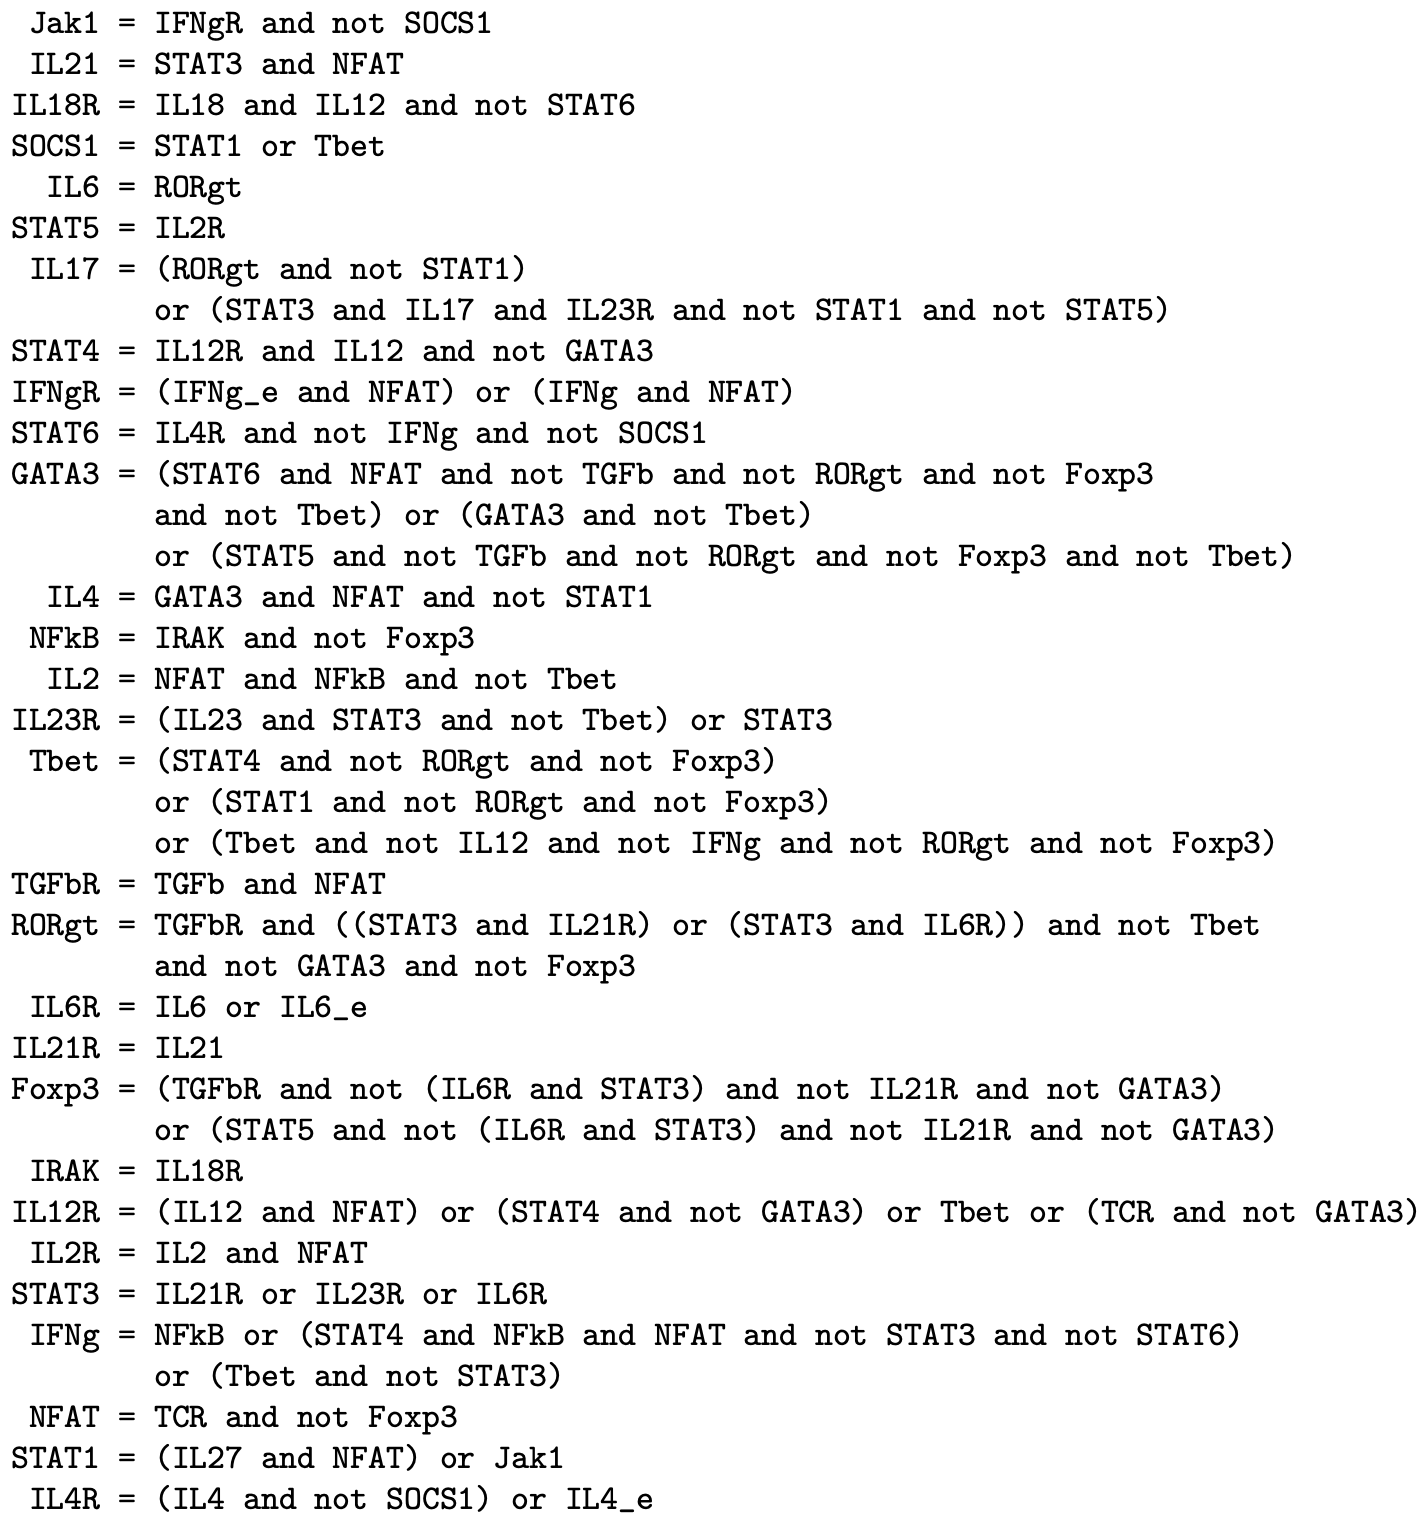
\includegraphics[width=0.49\textwidth]{figs-datamod2023/TcellBN.png}
	\end{center}
%\fontsize{8}{8}
%\begin{verbatim}
% Jak1 = IFNgR and not SOCS1 
% IL21 = STAT3 and NFAT
%IL18R = IL18 and IL12 and not STAT6 
%SOCS1 = STAT1 or Tbet 
%  IL6 = RORgt 
%STAT5 = IL2R 
% IL17 = (RORgt and not STAT1) 
%        or (STAT3 and IL17 and IL23R and not STAT1 and not STAT5) 
%STAT4 = IL12R and IL12 and not GATA3 
%IFNgR = (IFNg_e and NFAT) or (IFNg and NFAT) 
%STAT6 = IL4R and not IFNg and not SOCS1 
%GATA3 = (STAT6 and NFAT and not TGFb and not RORgt and not Foxp3 
%        and not Tbet) or (GATA3 and not Tbet) 
%        or (STAT5 and not TGFb and not RORgt and not Foxp3 and not Tbet) 
%  IL4 = GATA3 and NFAT and not STAT1 
% NFkB = IRAK and not Foxp3 
%  IL2 = NFAT and NFkB and not Tbet 
%IL23R = (IL23 and STAT3 and not Tbet) or STAT3 
% Tbet = (STAT4 and not RORgt and not Foxp3) 
%        or (STAT1 and not RORgt and not Foxp3) 
%        or (Tbet and not IL12 and not IFNg and not RORgt and not Foxp3) 
%TGFbR = TGFb and NFAT 
%RORgt = TGFbR and ((STAT3 and IL21R) or (STAT3 and IL6R)) and not Tbet 
%        and not GATA3 and not Foxp3 
% IL6R = IL6 or IL6_e 
%IL21R = IL21 
%Foxp3 = (TGFbR and not (IL6R and STAT3) and not IL21R and not GATA3) 
%        or (STAT5 and not (IL6R and STAT3) and not IL21R and not GATA3) 
% IRAK = IL18R 
%IL12R = (IL12 and NFAT) or (STAT4 and not GATA3) or Tbet or (TCR and not GATA3) 
% IL2R = IL2 and NFAT 
%STAT3 = IL21R or IL23R or IL6R 
% IFNg = NFkB or (STAT4 and NFkB and NFAT and not STAT3 and not STAT6) 
%        or (Tbet and not STAT3) 
% NFAT = TCR and not Foxp3 
%STAT1 = (IL27 and NFAT) or Jak1 
% IL4R = (IL4 and not SOCS1) or IL4_e 
%\end{verbatim}
	\caption{Boolean updates of the T Cell differentiation model from \cite{puniya2018mechanistic}, available at \cite{ModelCellCollective}.}
	\label{fig:boolean-formulas}
\end{figure}

\begin{figure}[t]
\begin{minipage}{0.9\linewidth}
\footnotesize
\begin{verbatim}
myreactions([
    react([stat5],[gata3,il21r,il6r],[foxp3]),
    react([stat5],[gata3,il21r,stat3],[foxp3]),
    react([tgfbr],[gata3,il21r,il6r],[foxp3]),
    react([tgfbr],[gata3,il21r,stat3],[foxp3]),
    react([gata3],[tbet],[gata3]),
    react([nfat,stat6],[foxp3,rorgt,tbet,tgfb],[gata3]),
    react([stat5],[foxp3,rorgt,tbet,tgfb],[gata3]),
    react([nfat,nfkb,stat4],[stat3,stat6],[ifng]),
    react([nfkb],[],[ifng]),
    react([tbet],[stat3],[ifng]),
    react([ifng,nfat],[],[ifngr]),
    react([ifnge,nfat],[],[ifngr]),
    react([il12,nfat],[],[il12r]),
    react([tbet],[],[il12r]),
    react([tcr],[gata3],[il12r]),
    react([il17,il23r,stat3],[stat1,stat5],[il17]),
    react([rorgt],[stat1],[il17]),
    react([il12,il18],[stat6],[il18r]),
    react([nfat,nfkb],[tbet],[il2]),
    react([nfat,stat3],[],[il21]),
    react([il21],[],[il21r]),
    react([il23,stat3],[tbet],[il23r]),
    react([stat3],[],[il23r]),
    react([il2,nfat],[],[il2r]),
    react([stat4],[gata3],[il2r]),
    react([gata3,nfat],[stat1],[il4]),
    react([il4],[socs1],[il4r]),
    react([il4e],[],[il4r]),
    react([rorgt],[],[il6]),
    react([il6],[],[il6r]),
    react([il6e],[],[il6r]),
    react([il18r],[],[irak]),
    react([ifngr],[socs1],[jak1]),
    react([tcr],[foxp3],[nfat]),
    react([irak],[foxp3],[nfkb]),
    react([il21r,stat3,tgfbr],[foxp3,gata3,tbet],[rorgt]),
    react([il6r,stat3,tgfbr],[foxp3,gata3,tbet],[rorgt]),
    react([stat1],[],[socs1]),
    react([tbet],[],[socs1]),
    react([il27,nfat],[],[stat1]),
    react([jak1],[],[stat1]),
    react([il21r],[],[stat3]),
    react([il23r],[],[stat3]),
    react([il6r],[],[stat3]),
    react([il12,il12r],[gata3],[stat4]),
    react([il2r],[],[stat5]),
    react([il4r],[ifng,socs1],[stat6]),
    react([stat1],[foxp3,rorgt],[tbet]),
    react([stat4],[foxp3,rorgt],[tbet]),
    react([tbet],[foxp3,ifng,il12,rorgt],[tbet]),
    react([nfat,tgfb],[],[tgfbr]) ]).
    
\end{verbatim}
\end{minipage}
\caption{\BioResolve implementation of the T cell case study from \Cref{sec:datamod2023}.}
\label{fig:bioresolve:tcell}
\end{figure}

\subsection{Auxiliary Material for the \GROOVE experiments}\label{app:groove}

To replicate the \GROOVE experiments reported in \Cref{sec:RS2GTS} (for the toy running example) and \Cref{sec:experiments}, we have included the following supplementary resources with this submission:
\begin{itemize}
\item The rule systems described in \Cref{sec:RS2GTS};
\item The start graphs derived from the \BioResolve specifications in this appendix (\ref{app:running}--\ref{app:maude});
\item Instructions for calling the \GROOVE generator so as to reproduce all the exploration runs, occurrence graphs and model checking results (using \href{https://github.com/nl-utwente-groove/code/releases/tag/release-7_4_3}{\GROOVE version 7.4.3}).
\end{itemize}

